\documentclass[12pt]{article}
\usepackage{graphicx}
\usepackage{wrapfig}
\usepackage{subfigure}
\usepackage{multirow}
\usepackage{hyperref}
\usepackage{amsmath}
\usepackage{amssymb}
%\usepackage{ngerman}
\usepackage[ansinew]{inputenc}
\usepackage[left=2cm,top=1cm]{geometry}

% vector graphics test
\usepackage{color}
\usepackage{transparent}
\graphicspath{{graphs/}}

\setlength{\parindent}{0pt}

%\usepackage[outdir=./]{epstopdf}
%\epstopdfsetup{outdir=./}


\begin{document}
	\pagestyle{empty}
	

\begin{titlepage}
	\centering
	\bigskip
	\huge{Astronomisches Praktikum:\\Spektrale Klassifikation extragalaktischer Objekte}\\
	\bigskip
	\large{Versuch 10}\\
	\bigskip
	\large{Jan R\"{o}der \& Julia Lienert}
	\bigskip
	\tableofcontents
\end{titlepage}

\pagebreak


\section{Einleitung}

Um festzustellen, welcher Klasse eine Galaxie angeh\"{o}rt, kann man ihr Strahlungsspektrum aufnehmen und die Fl\"{u}sse und Breiten der Linien analysieren. Bildet man bestimmte Verh\"{a}ltnisse dieser Linien, lassen sie sich in die sogenannten diagnostischen Diagramme eintragen. In diesen Diagrammen entsteht dann eine bestimmte Kurve, die die aktiven von den normalen Galaxien separiert.\\
Aktive Galaxien teilen sich wiederum auf in Untergruppen, die f\"{u}r sich spezielle charakteristische Eigenschaften haben. Grunds\"{a}tzlich unterteilt man in Seyfert-Typen, die sich phsykalisch eigentlich nur in der gemoetrischen Orientierung zu uns unterscheiden. Alle Seyfert-Galaxien zeichnen sich durch eine nicht durch Sterne erkl\"{a}rbare, auf weniger als 0.01\,pc konzentrierte Energiequelle aus. Seyfert 2-Galaxien erscheinen uns mit Linienbreiten \"{a}hnlich denen der verbotenen \"{U}berg\"{a}nge.\\
Die ersten, die Galaxien in diagnostische Diagramme einf\"{u}gten, waren Veilleux und Osterbrock 1987. Die Separation von Galaxientypen in dieses Diagrammen liegt daran, dass Elemente in einem aktiven Galaxienkern st\"{a}rker ionisiert werden, als wenn nur Sterne als Strahlungsquelle dienen.

\section{Spektrografie}

\subsection{Aufgabe 1}

\begin{figure} [h]
	\centering
	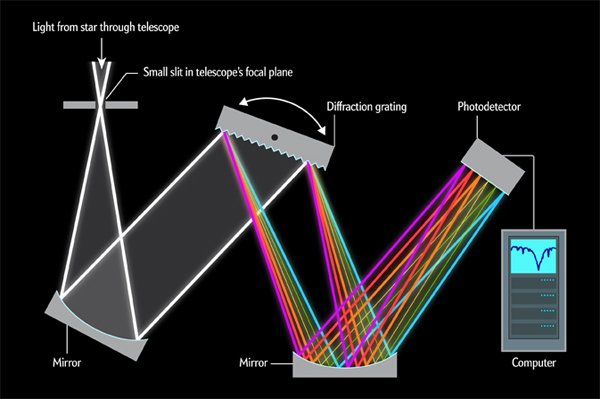
\includegraphics[width=0.8\textwidth]{spectrograph.jpg}
	\caption{Schematischer Aufbau eines Spektrographen}
	\label{fig:spektrograf}
\end{figure}

Abbildung \ref{fig:spektrograf} zeigt den schematischen Aufbau eines Spektrographen. Licht f\"{a}llt durch das Objektiv des Teleskops, wo es durch einen Hauptspiegel auf ein Gitter projiziert wird. Dieses Gitter hat Dispersionseingenschaften, wodurch das Licht in seine Bestandteile zerlegt wird. Das Aufgespaltene Licht f\"{a}llt nun auf einen zweiten Spiegel, der das Licht gerade so auf einen Detektor reflektiert, dass die Farben ``geordnet'' dort auftreffen. Je nach Wellenl\"{a}ngenbereich kann der Detektor eines anderen Typs sein.  Die Rotationsm\"{o}glichkeit des Gitters bestimmt, welche Wellenl\"{a}ngen des einfallenden Lichts \"{u}berhaupt bis zum Detektor kommen.

\subsection{Aufgabe 2}

Eine Linie oder einen \"{U}bergang nennt man ``verboten'', wenn er im Labor nicht erzeugbar ist, er aber dennoch beobachtet wird. Oft treten diese Linien in Gasen geringer Dichte auf, wo St\"{o}sse mit anderen Molek\"{u}len unwahrscheinlich sind. Wird dann ein Gasteilchen auf ein h\"{o}heres Energieniveau gehoben, wird der \"{U}bergang zur\"{u}ck in den Grundzustand als ein verbotener \"{U}bergang erfolgen. Beispiele sind z. B. die O[III]-Linie bei etwa 500\,nm oder die 21\,cm-Linie des Wasserstoffs.


\section{Analyse eines Galaxien-Spektrums mit IRAF}

\begin{table} [h]
	\centering
	\begin{tabular}{|c|c|}
		\hline
		Linie	  & Wellenl\"{a}nge [\AA{}]			\\ \hline
		[O\,III]  & 5007 \\ \hline
	    H$\beta$  & 4861 \\ \hline
	    H$\alpha$ & 6563 \\ \hline
	    [N\,II]   & 6583 \\ \hline
	    [S\,II]   & 6721 \\ \hline
	    [O\,I]    & 6300 \\ \hline
	\end{tabular}
	\caption{Ruhewellenl\"{a}ngen}
	\label{tab:lambda}
\end{table}

\subsection{Aufgabe 1}

Im Datenset ist die Wellenl\"{a}nge $\lambda$ auf der x-Achse aufgetragen. Zuerst wird \textit{o1.fits} aufgerufen und die [O\,III]-Linie identifiziert, und zwar zu 5376.65\,\AA{}. Mit der Ruhewellenl\"{a}nge aus \ref{tab:lambda} sowie
\begin{equation}
	\frac{\lambda}{\lambda_0} = 1+z
\end{equation}
erh\"{a}lt man $z=0.074$. 

\subsection{Aufgabe 3}
Fittet man in jedem Spektrum die markanten Linien mit einer Gauss-Kurve und tr\"{a}gt immer den Fluss und die FWHM in eine Tabelle ein, so kann man die Logarithmen bestimmter Flussverh\"{a}ltnisse bestimmen, um die Galaxien in die vorliegenden diagnostischen Diagramme einzutragen. Da in \textit{o1.fits} keine [N\,II]-Linie vorhanden war, beginnen die Nummern bei 2. Nummer 3 fehlt ebenfalls, da zwar [O\,III] und H$\beta$ sichtbar waren, die anderen jedoch ausserhalb des gespeicherten Spektrums lagen. \\

\begin{figure} [h]
	\centering
	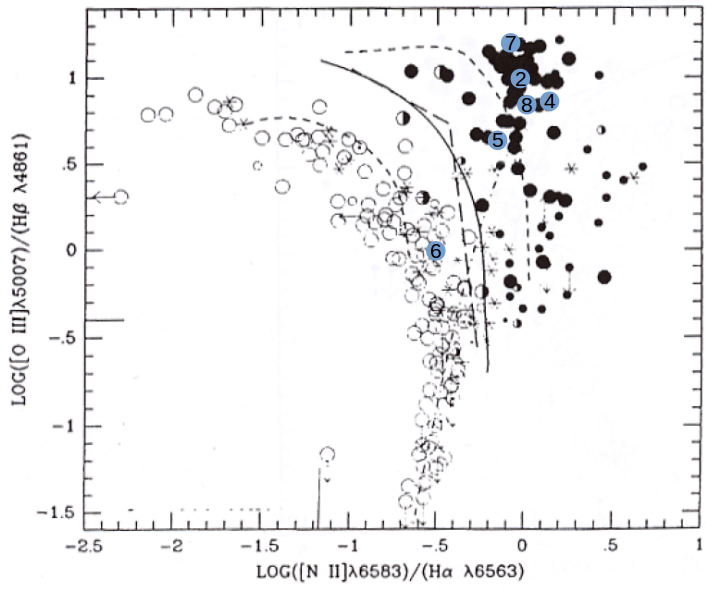
\includegraphics[width=0.8\textwidth]{N2}
	\caption{Diagnostisches Diagramm 1}
	\label{fig:n2}
\end{figure}
\begin{figure} [h]
	\centering
	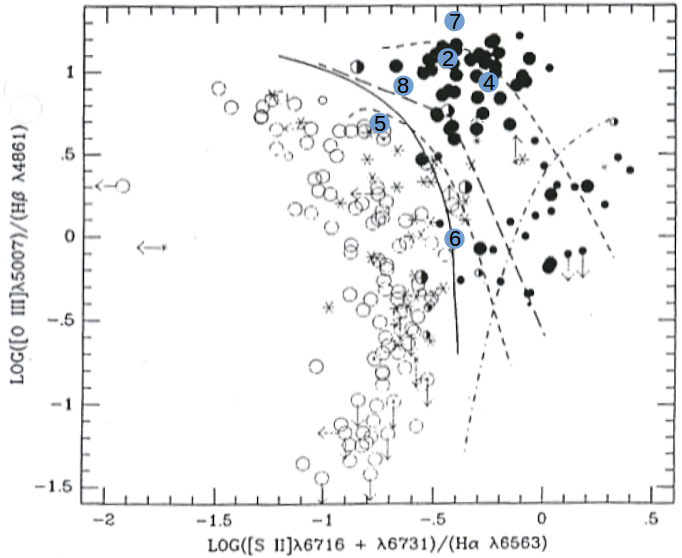
\includegraphics[width=0.8\textwidth]{S2}
	\caption{Diagnostisches Diagramm 2}
	\label{fig:s2}
\end{figure}
\begin{figure} [h]
	\centering
	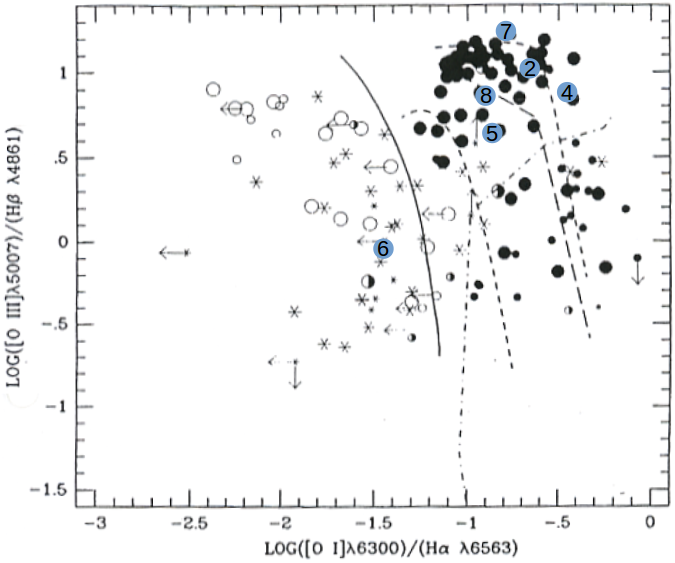
\includegraphics[width=0.8\textwidth]{O1}
	\caption{Diagnostisches Diagramm 3}
	\label{fig:o1}
\end{figure}

\section{Diskussion}

Der Versuch bestand haupts\"{a}chlich aus der Arbeit mit dem Analyseprogramm IRAF. Damit war es sehr leicht m\"{o}glich, Linien zu identifizieren und Gauss-Fits anzulegen. Danach wurden die logarithmierten Flussverh\"{a}ltnisse mit Excel berechnet und in die diagnostischen Diagramme eingetragen. Dabei fiel auf, dass Galaxie Nummer 6 anscheinend keine aktive Galaxie ist, da sie in den Diagrammen 1 und 3 deutlich linksseitig der separierenden Kurven liegt. \\
Bei Galaxien wie Nummer 2, 5, 6 oder 8 war gut zu erkennen, dass die FWHM derjenigen der [O\,III]-Linie dehr nahe kommen und folglich vermutlich Seyfert 1-Galaxien sind.


% o2: S1
% o4: 
% o5: S1
% o6: S1
% o7:
% o8: S1



\section{Quellen}
\begin{enumerate}
	\item Versuchsanleitung zu Versuch 10
\end{enumerate}


%\begin{figure} [h]
%	\centering
%	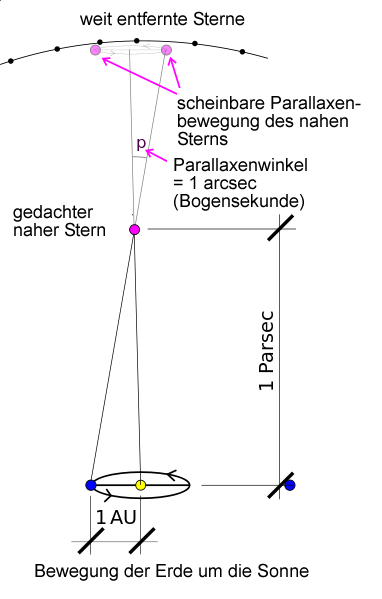
\includegraphics[width=0.4\textwidth]{2_4_Parallaxe.png}
%	\caption{Skizze zur Erkl�rung der Parallaxe (entnommen aus [2])}
%	\label{fig:Parallaxe}
%\end{figure}








\end{document}